%% The following is a directive for TeXShop to indicate the main file
%%!TEX root = report.tex

\chapter{Results}
\label{ch:Results}

\section{Intel Memory Latency Checker}

The measurements in this section were collected using the Intel Memory Latency Checker, a tool
developed by Intel to evaluate memory bandwidth and latency.  Version 3.5 includes explicit
support for evaluating DRAM and NVM.  It is NUMA aware and can be used for evaluating both
node-local as well as node-remote memories.~\cite{IntelMLC35}

I note that the provided documentation for this tool does not describe some modes of
this tool that are, in fact, used in this evaluation.  Further, actually enabling the
correct testing mode for NVM is not easy to reproduce from the information available.
Thus, when reporting specific results I have included the command line switches used
as part of the testing. 

The tests considered in this section all used a zero injection latency (\texttt{-d0},)
as this represents the highest workload against the given memory --- latency injection
provides a simple mechanism for evaluating performance on workloads that are not
pushing the bandwidth boundary.  While I did perform evaluations with higher
injection rates, I have chosen to omit that additional data from this report.

Each specific test run uses various flags to control the behavior.  Unless
otherwise noted, all tests used the \verb+--loaded_latency+ option, which
means that the test utility is measuring the latency of the memory with
some load imposed.

Note that for all tests, \textbf{core 0} is used for measurements.  Thus, when
we report 3 cores in use, two of them are generating load and one is performing
the latency measurements.

For the various tests I use the switches as shown in Table \ref{mlc:switches}

\begin{table}\label{mlc:switches}
    \caption{MLC switches used during testing}
    \begin{tabular}{@{}clc@{}}
        Switch & Effect & See Section \\ \toprule
        \verb+-d+ & Latency injection (seconds) &  \\
        \verb+-t+ & Test time (seconds) &  \\
        \verb+-l+ & Stride size (bytes) & \\
        \verb+-R+ & Read-only workload & \ref{baseline:dram}, \ref{baseline:nvm} \\
        \verb+-W2+ & Read-Write 2:1 Workload &  \\ \bottomrule
    \end{tabular}%
\end{table}

Note that reported stride sizes were 16, 32, 64, 128, 256, 512, 1024, and 2048 in all cases.
In a few cases I report 4096, but for many tests that stride size failed to work properly
with the given test.  Similarly, I tested sizes below 16 bytes but found that it frequently
failed.

\subsection{Baseline Measurements}

This section describes the information for \textbf{non-temporal move} operations on the same node. Because
these are done as non-temporal move operations, they bypass the cache and write directly to the actual
memory.  Note that the failure domain is discussed in greater detail in \S \ref{section:model:failure}.
The transfer involved here is sufficiently large that the impact of the memory controller caching
does not impact behavior.

\subsubsection{DRAM}\label{baseline:dram}

\begin{figure}
    \centering
    \caption{Baseline Measurement of DRAM Non-Temporal Write on the same NUMA Node}\label{chart:baseline:dram}
    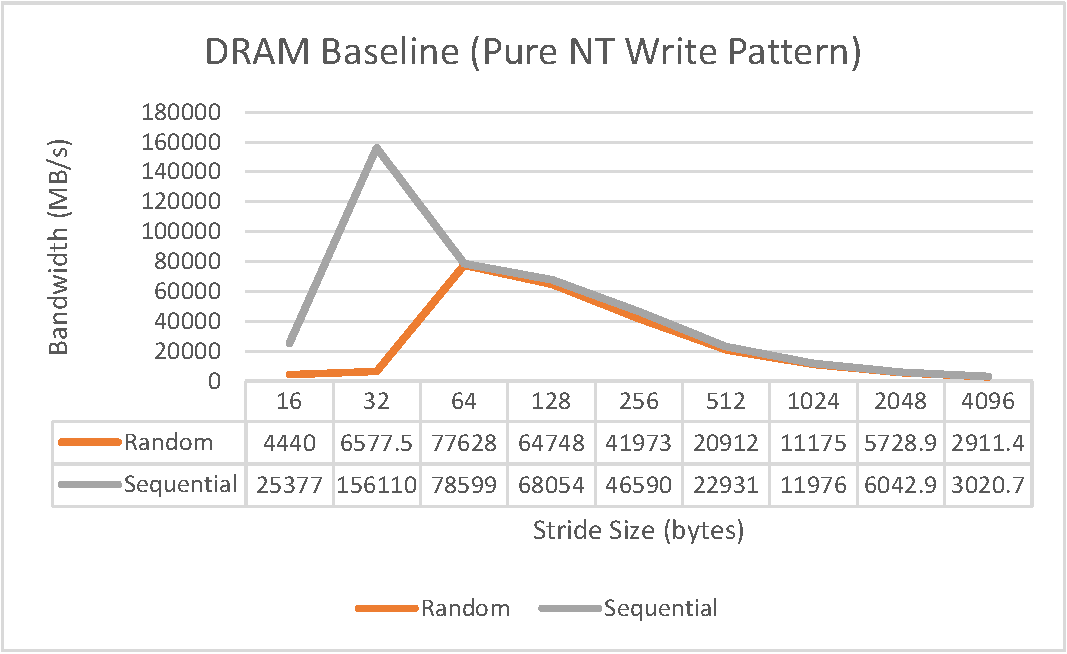
\includegraphics[width=1\textwidth]{charts/dram-baseline-nt-write-same-node-crop.pdf}
\end{figure}

Baseline testing was done using the switches:

\begin{verbatim}
    --loaded_latency -d0 -t10 -W6 -l1024 -T 
        -odata/bw_ctl_pmem0p1_seq_W6-0_23_400000_dram.dat
\end{verbatim}

The file \verb+data/bw_ctl_pmem0p1_seq_W6-0_23_400000_dram.dat+ contained the confirmation information
for the specific test layout:

\begin{verbatim}
0       W6 seq 400000 dram 0
1-23    W6 seq 400000 dram 0
\end{verbatim}

This drives the test to use core 0 for latency measurements, and cores 1-23 for load generation.

Note that the \verb+-l+ option was varied depending upon the ``stride'' size (unit of data handling).
The control file specified the disposition of the individual CPUs

I do not report results for any other DRAM tests.

Results for this test are showin in Figure \ref{chart:baseline:dram}.

\subsubsection{NVM}\label{baseline:nvm}

\begin{figure}[b]
\centering
    \caption{Baseline Measurement of NVM Non-Temporal Write on the same NUMA Node}\label{chart:baseline:nvm}
    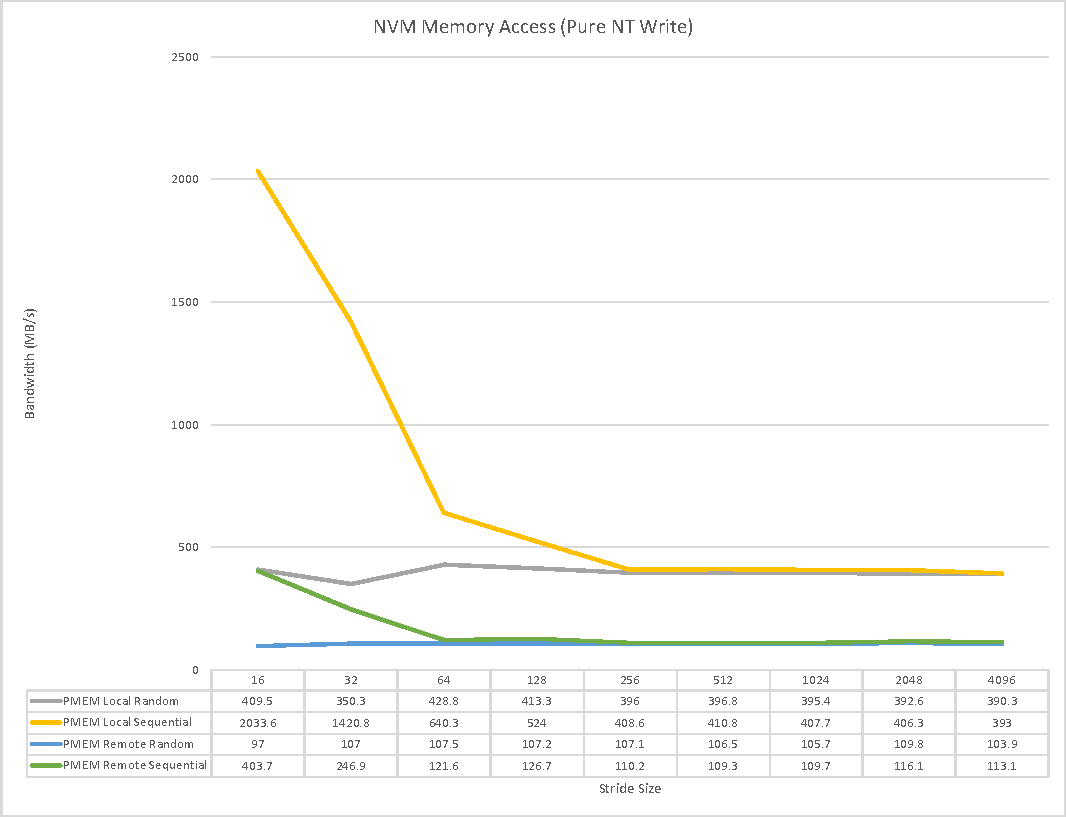
\includegraphics[width=1\textwidth]{charts/nt-write-both-nodes-crop.pdf}
\end{figure}

Baseline testing was done using the switches:

\begin{verbatim}
    --loaded_latency -d0 -t10 -W6 -l64 \
      -odata/bw_ctl_pmem0p1_seq_W6-0_23_400000_pmem.dat}
\end{verbatim}

The file \verb+data/bw_ctl_pmem0p1_seq_W6-0_23_400000_dram.dat+ contained the confirmation information
for the specific test layout:

\begin{verbatim}
0    W6 seq 400000 pmem /mnt/pmem0p1
1-23 W6 seq 400000 pmem /mnt/pmem0p1
\end{verbatim}

The \verb+pmem+ directive is used to put the test utility into ``persistent memory'' testing mode.
The final value is the name of the directory to use.  It \textbf{must} be a persistent memory
to run this test.  Otherwise the test will refuse to run.


\subsection{Cached Read}\label{mlc:r}

\subsubsection{Random Read}
\begin{figure}
    \centering
    \caption{Random Read (R)}\label{chart:random:read}
    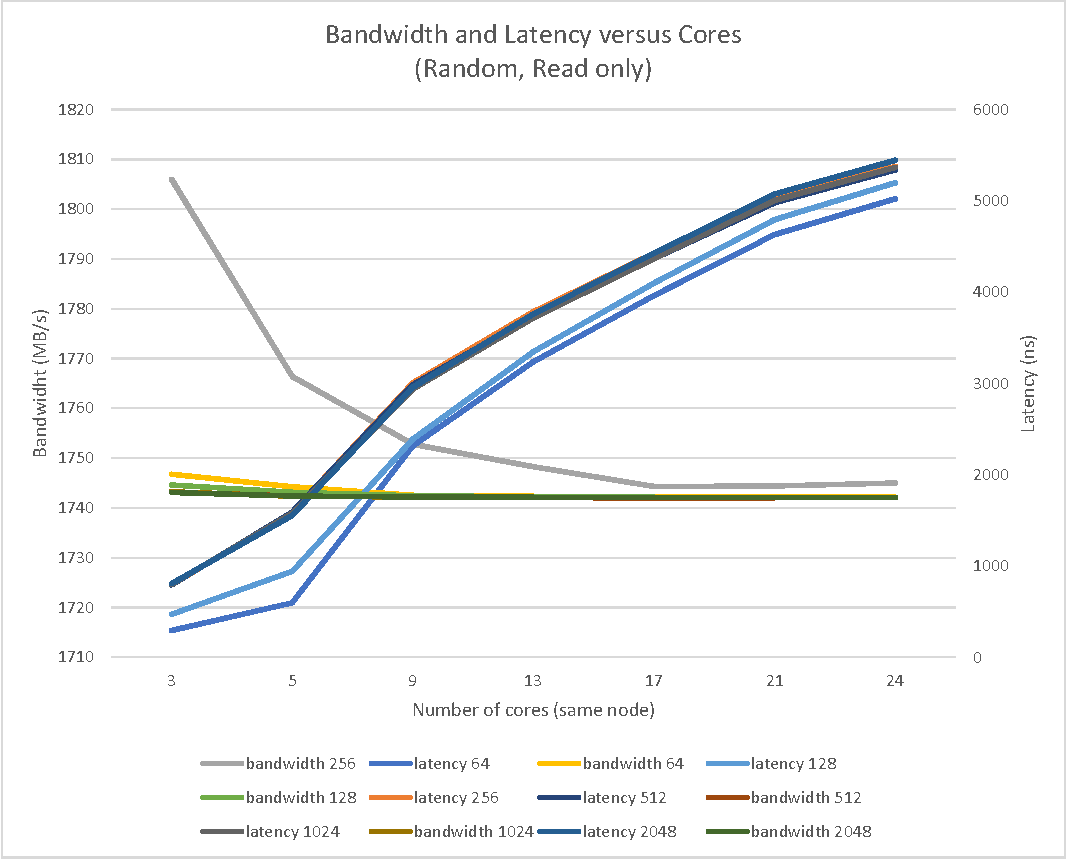
\includegraphics[width=1.25\textwidth, trim=3cm 0 0 0]{charts/random-r-crop.pdf}
\end{figure}

\begin{figure}
    \centering
    \caption{Sequential Read (R)}\label{chart:sequential:read}
    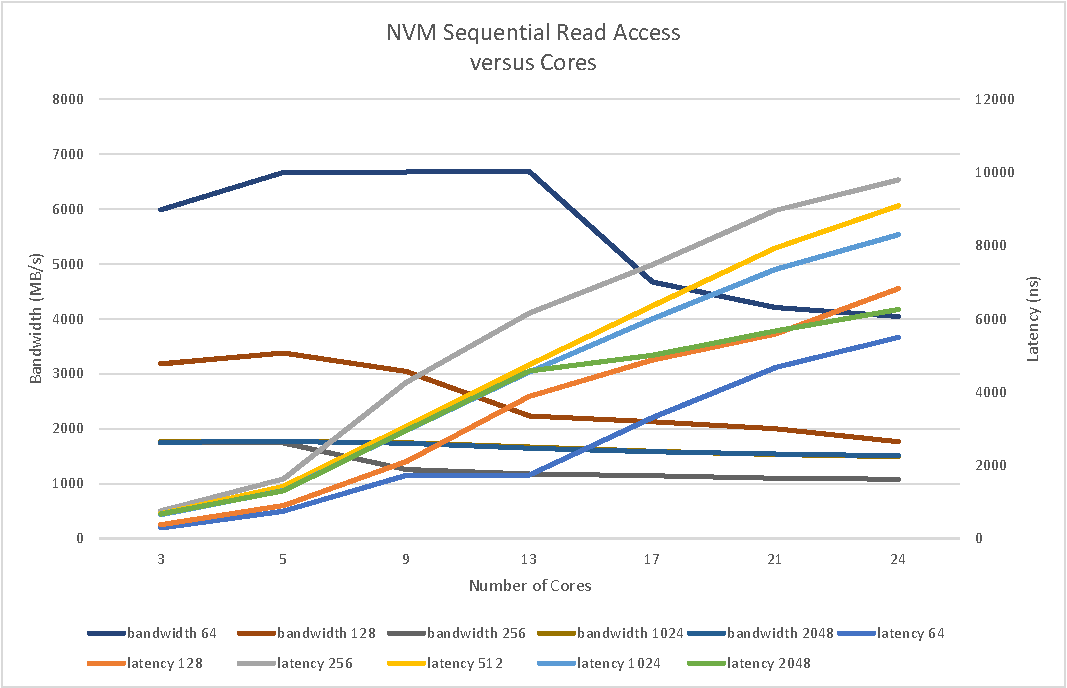
\includegraphics[width=1.25\textwidth, trim=3cm 0 0 0]{charts/sequential-r-crop.pdf}
\end{figure}

\begin{figure}
    \centering
    \caption{Random 2:1 Read/Write (W2)}\label{chart:random:w2}
    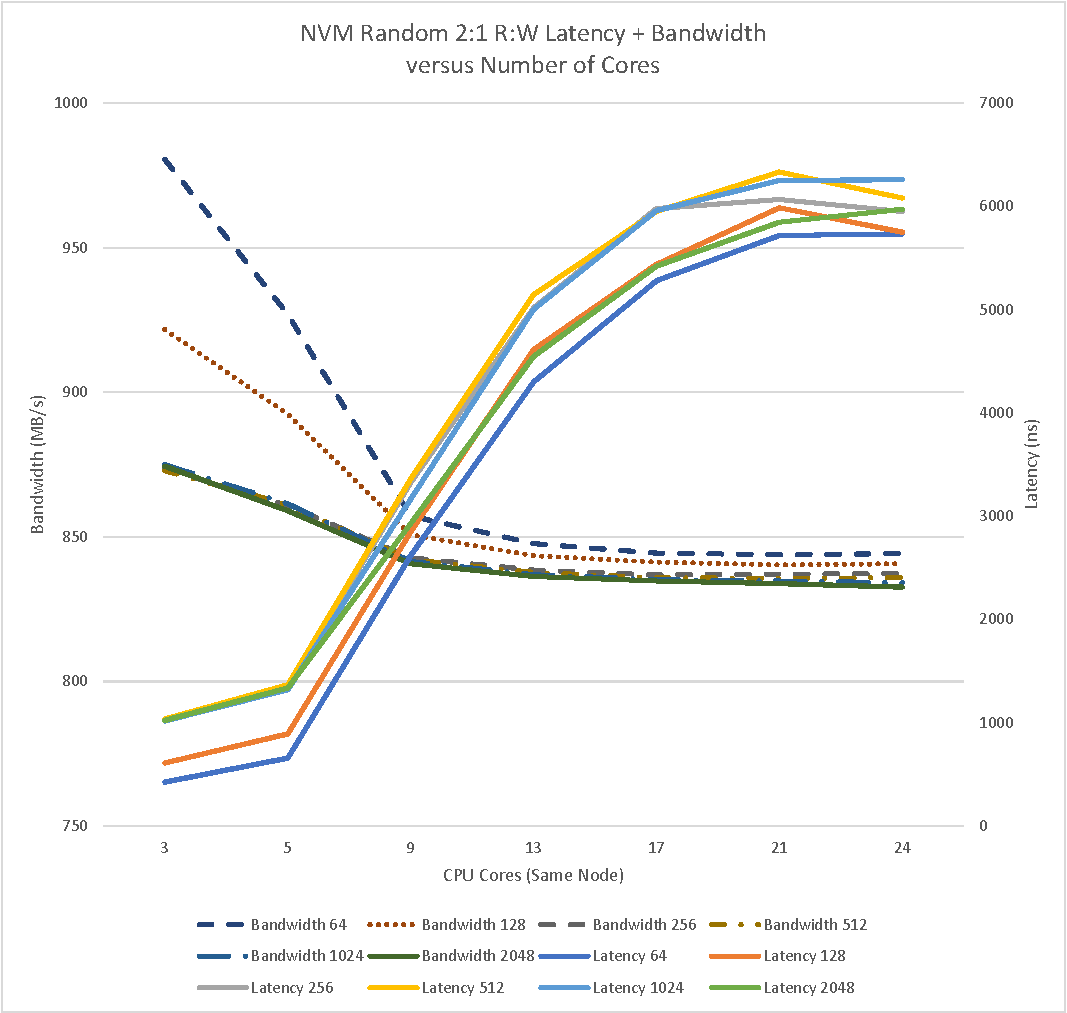
\includegraphics[width=1.25\textwidth,trim=3cm 0 0 0]{charts/random-w2-crop.pdf}
\end{figure}

\begin{figure}
    \centering
    \caption{Sequential 2:1 Read/Write (W2)}\label{chart:sequential:w2}
    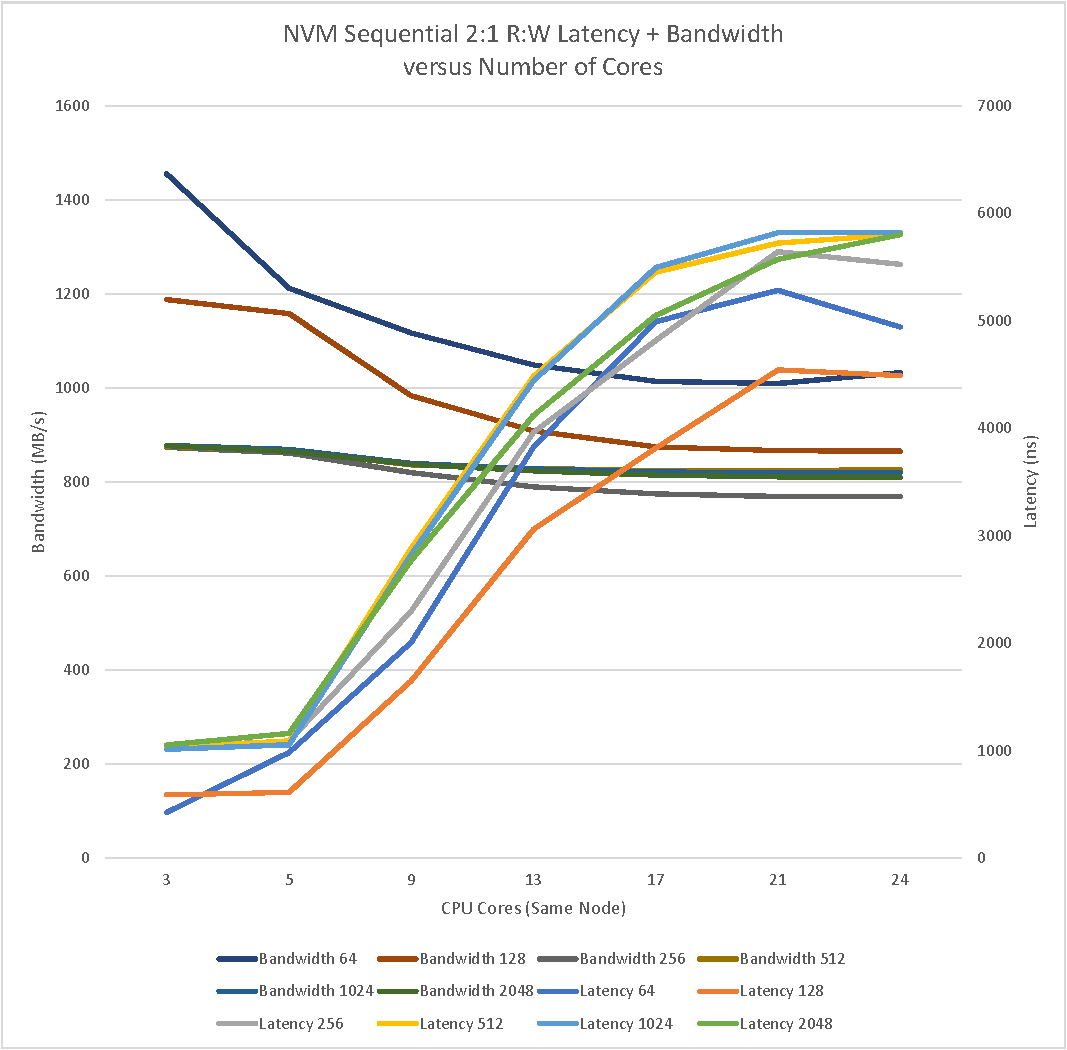
\includegraphics[width=1.25\textwidth,trim=3cm 0 0 0]{charts/sequential-w2-crop.pdf}
\end{figure}

\begin{figure}
    {\centering
    \caption{Sequential 3:1 Read/Write (W3)}\label{chart:sequential:w3}
    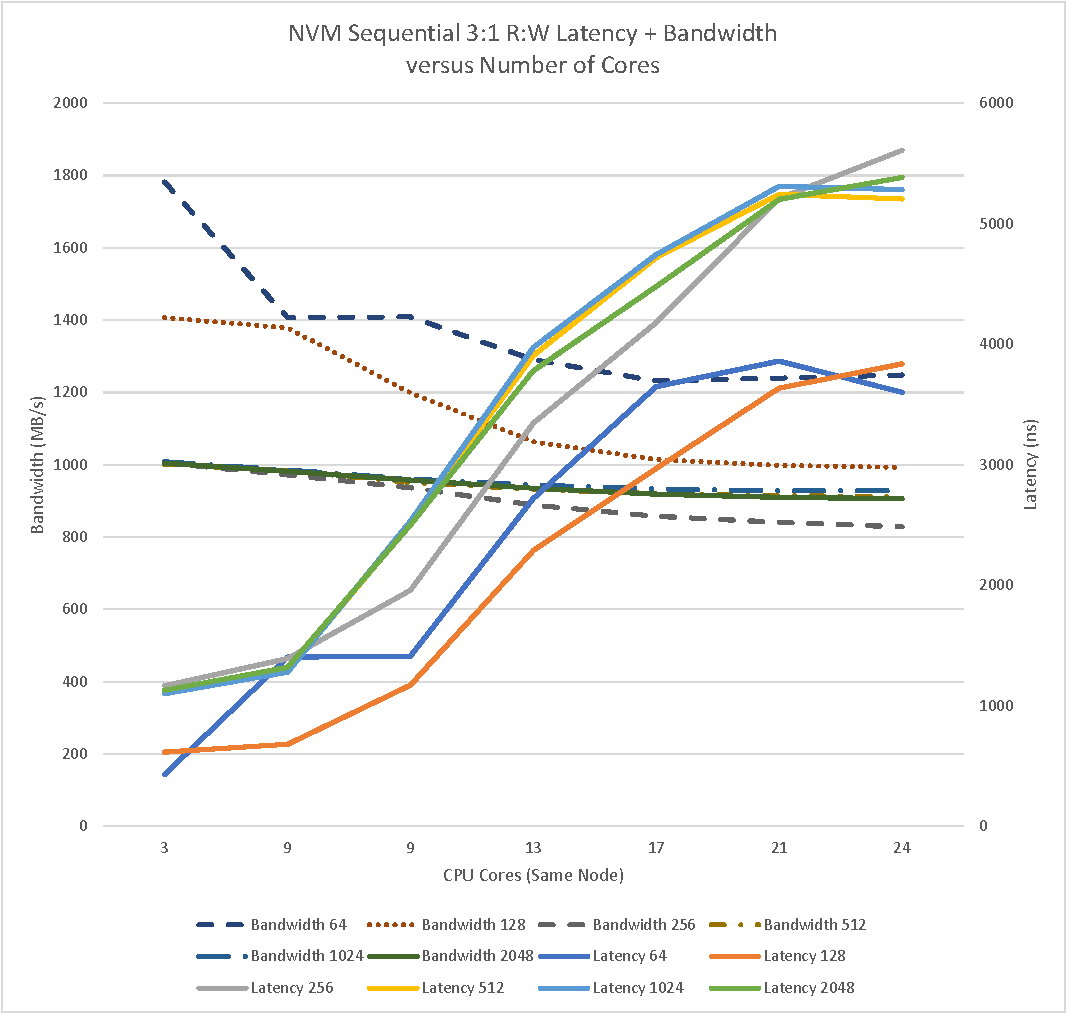
\includegraphics[width=0.45\textwidth]{charts/sequential-w3-crop.pdf}
    }
\end{figure}



\begin{figure}
    \centering
    \caption{To Be Captioned} %\label{chart:to-be-labeled}
    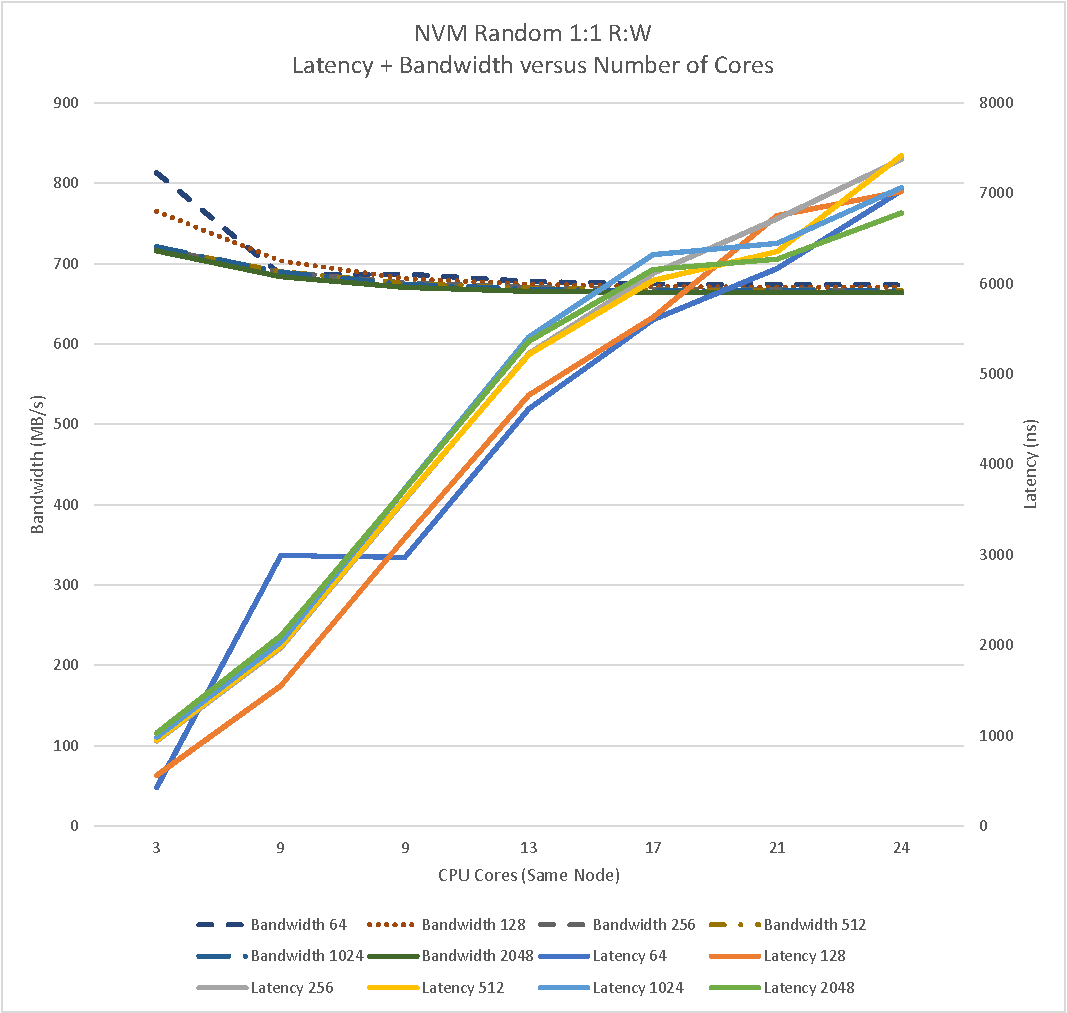
\includegraphics[width=0.45\textwidth]{charts/random-w5-crop.pdf}
\end{figure}





\begin{figure}
    \centering
    \caption{To Be Captioned} %\label{chart:to-be-labeled}
    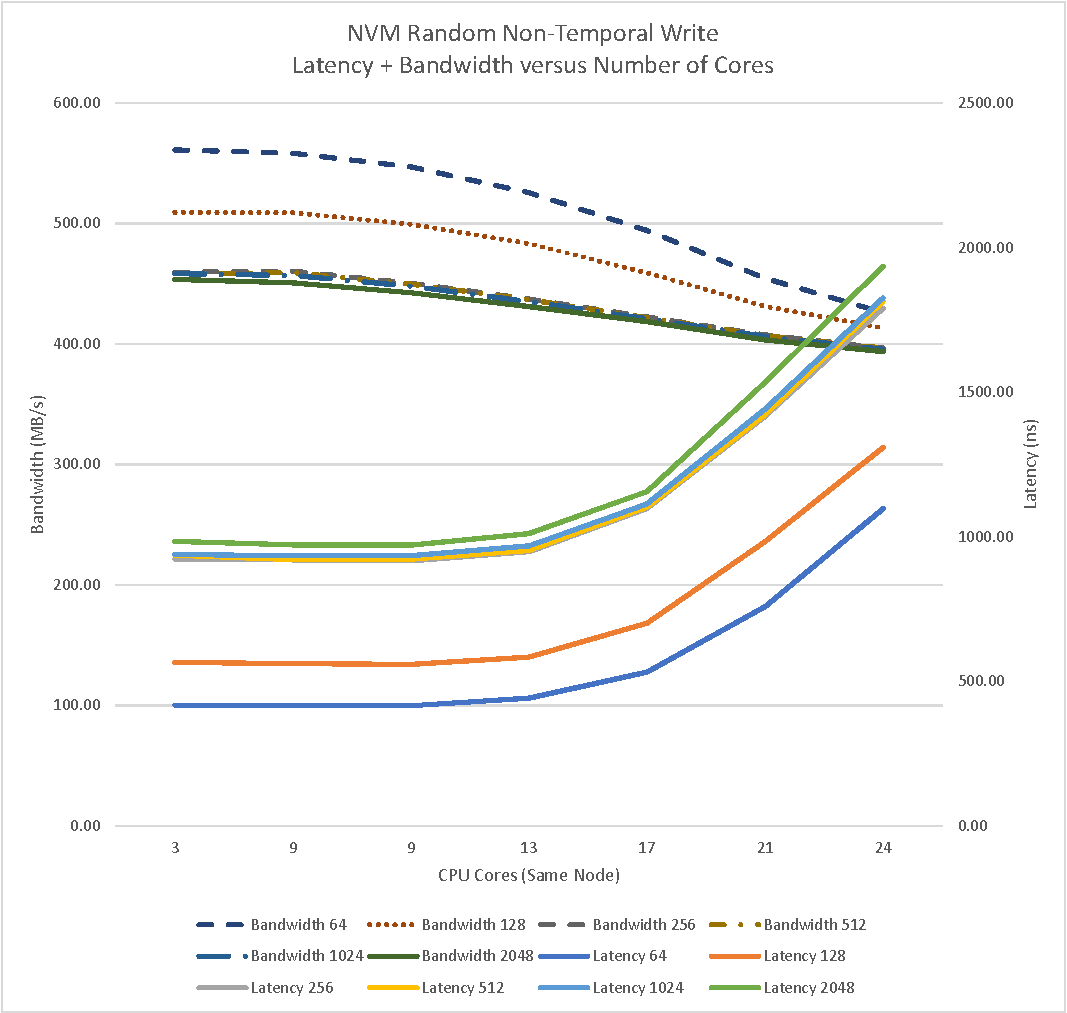
\includegraphics[width=0.45\textwidth]{charts/random-w6-crop.pdf}
\end{figure}

\begin{figure}
    \centering
    \caption{To Be Captioned} %\label{chart:to-be-labeled}
    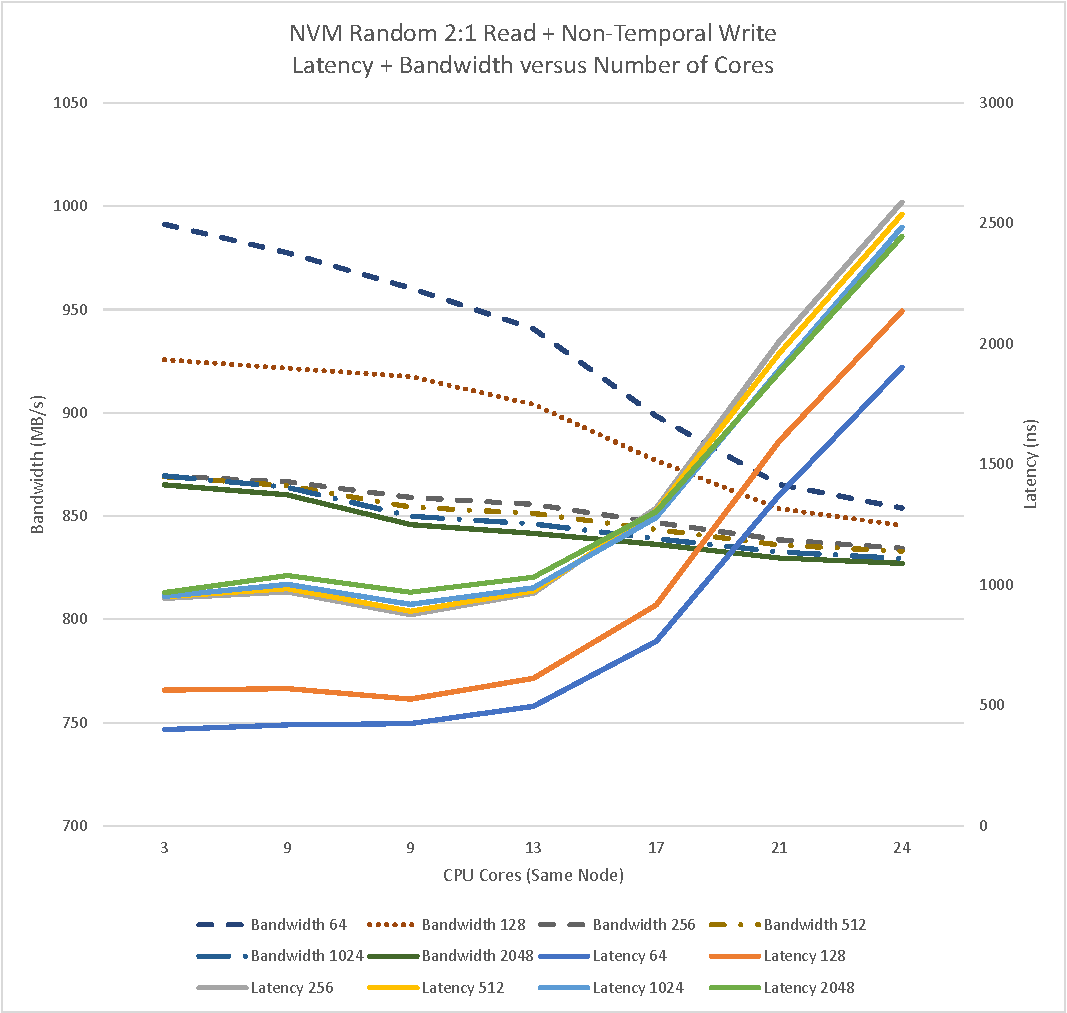
\includegraphics[width=0.45\textwidth]{charts/random-w7-crop.pdf}
\end{figure}

\begin{figure}
    \centering
    \caption{To Be Captioned} %\label{chart:to-be-labeled}
    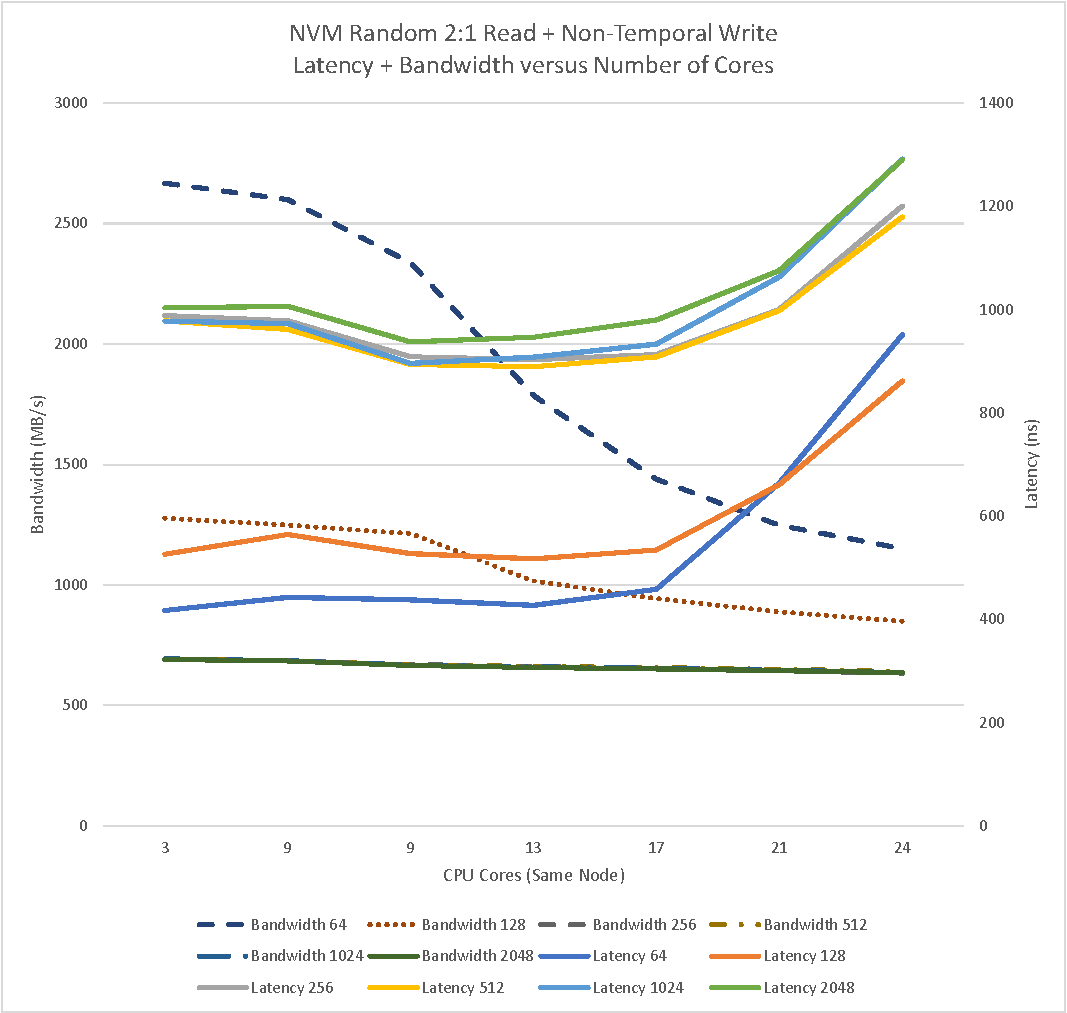
\includegraphics[width=0.45\textwidth]{charts/random-w8-crop.pdf}
\end{figure}

\begin{figure}
    \centering
    \caption{To Be Captioned} %\label{chart:to-be-labeled}
    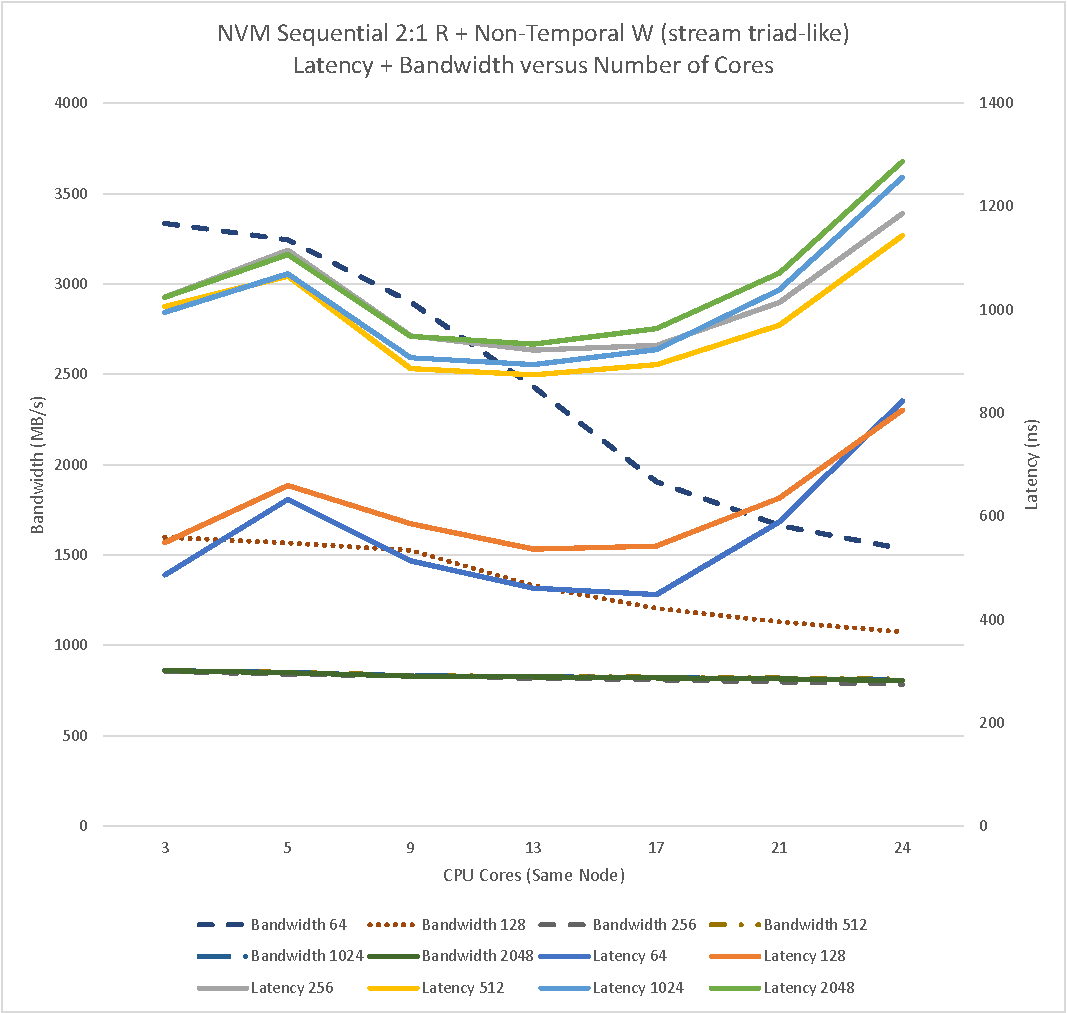
\includegraphics[width=0.45\textwidth]{charts/sequential-w10-crop.pdf}
\end{figure}




\begin{figure}
    \centering
    \caption{To Be Captioned} %\label{chart:to-be-labeled}
    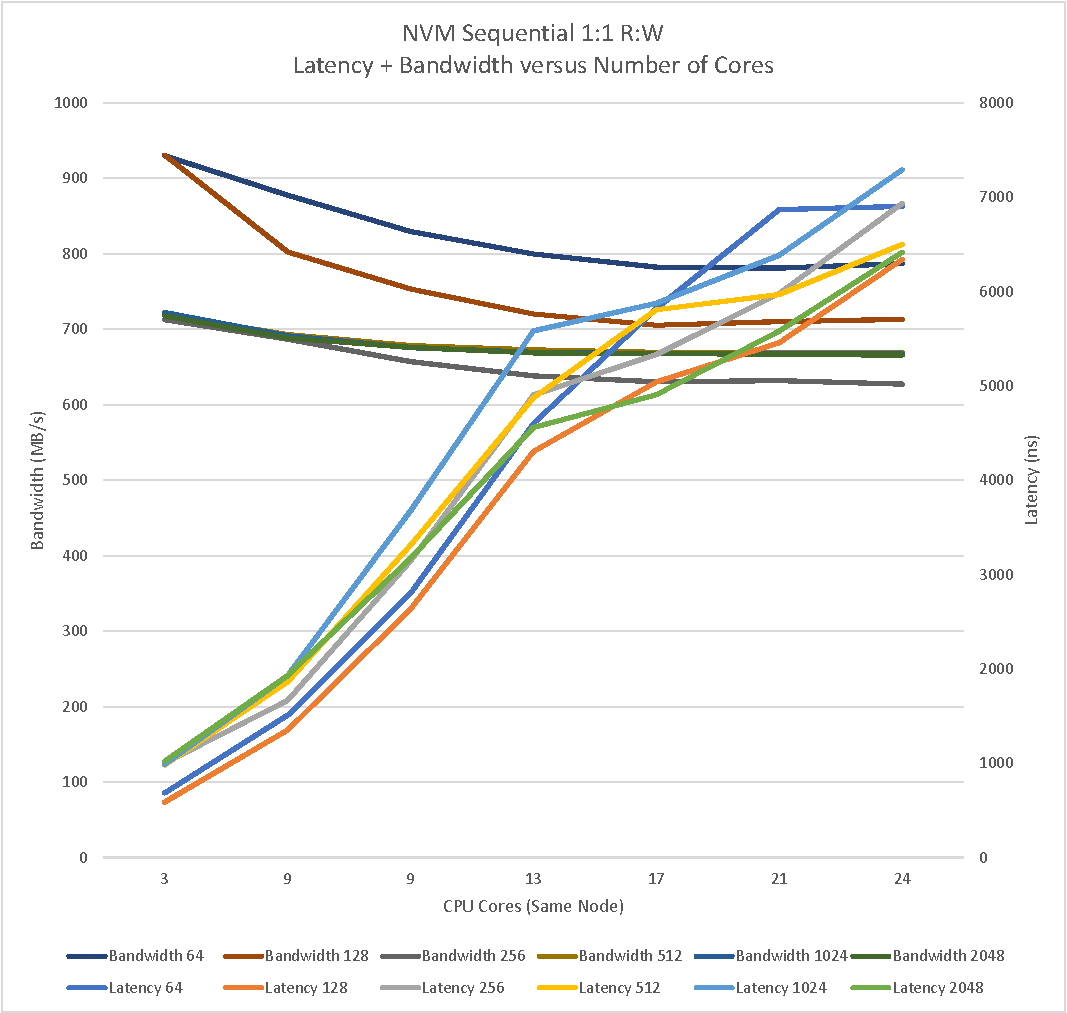
\includegraphics[width=0.45\textwidth]{charts/sequential-w5-crop.pdf}
\end{figure}


\begin{figure}
    \centering
    \caption{To Be Captioned} %\label{chart:to-be-labeled}
    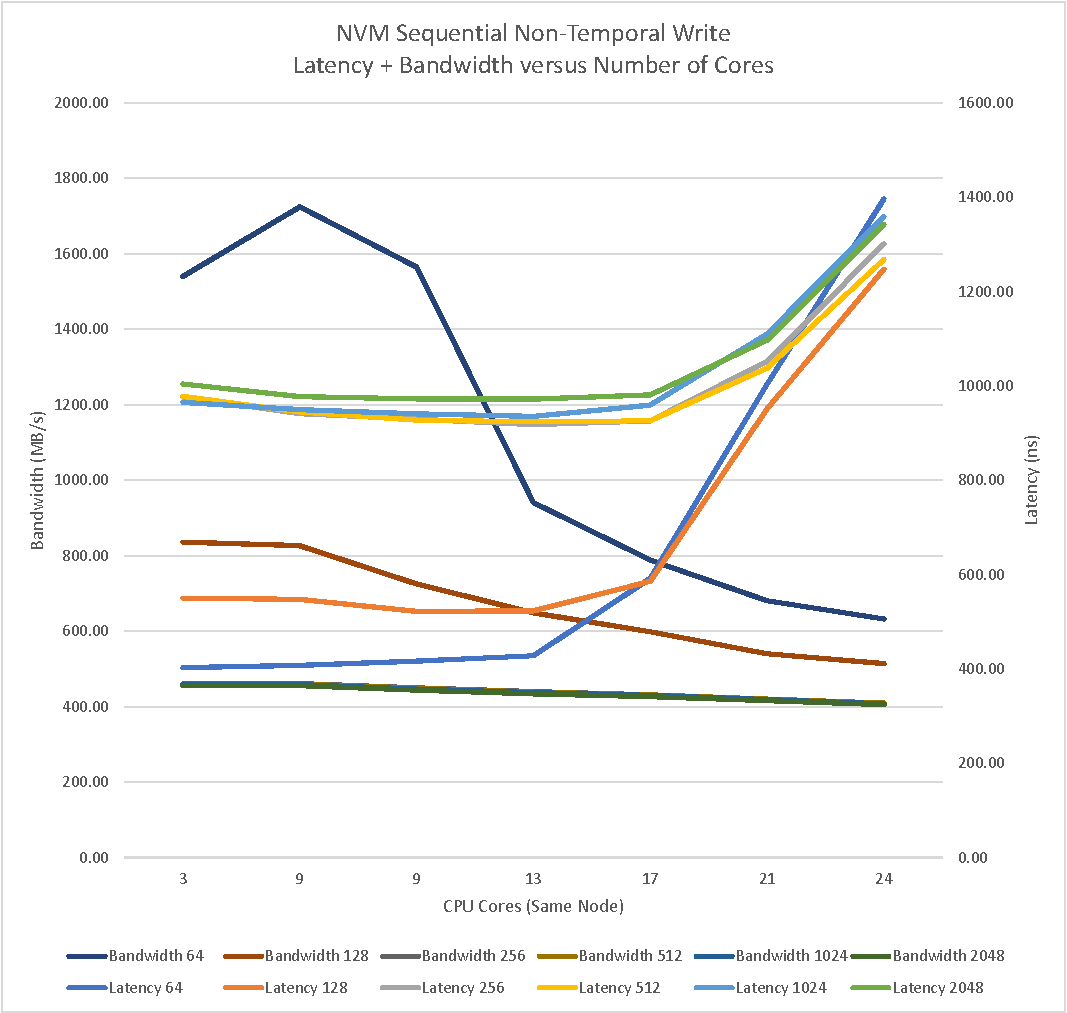
\includegraphics[width=0.45\textwidth]{charts/sequential-w6-crop.pdf}
\end{figure}


\begin{figure}
    \centering
    \caption{To Be Captioned} %\label{chart:to-be-labeled}
    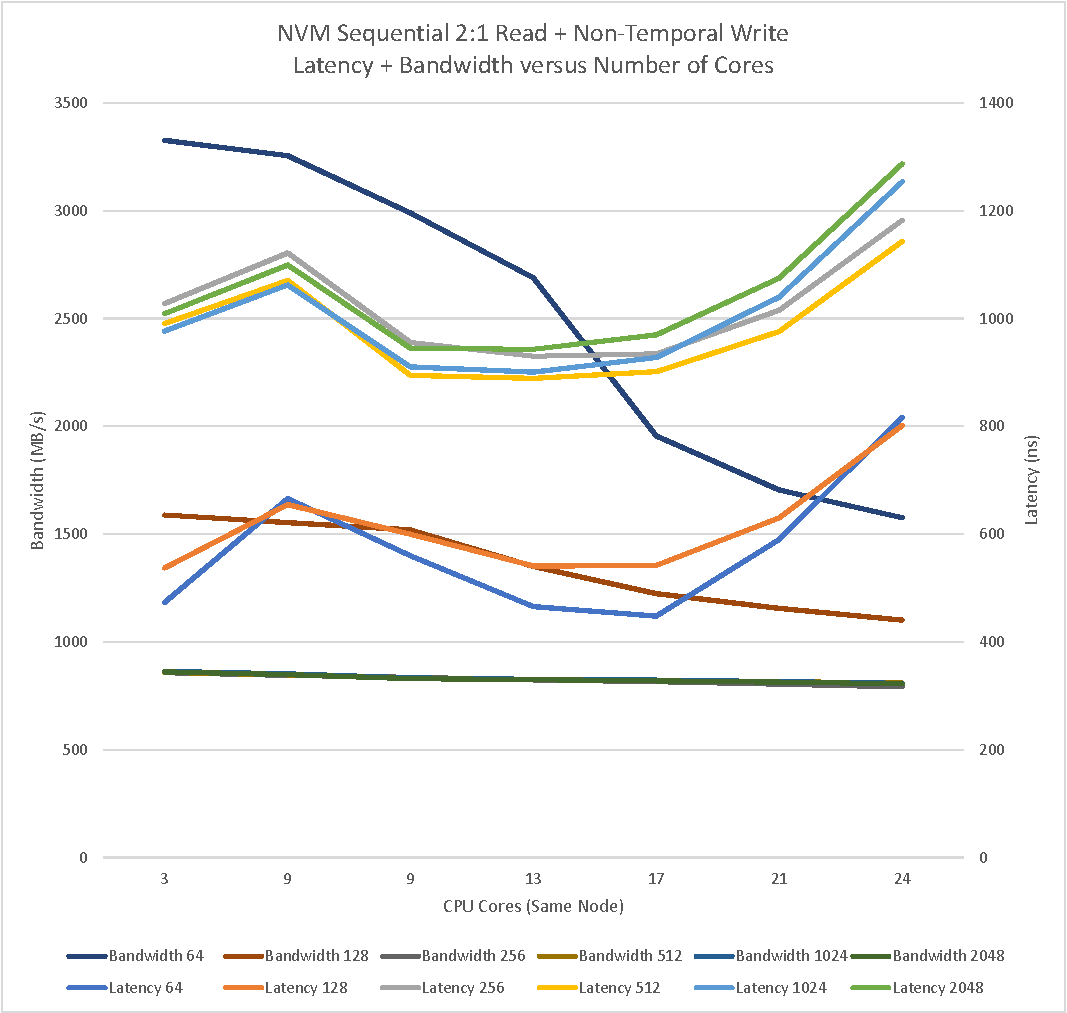
\includegraphics[width=0.45\textwidth]{charts/sequential-w7-crop.pdf}
\end{figure}

\endinput

\begin{figure}
    \centering
    \caption{To Be Captioned} %\label{chart:to-be-labeled}
    \includegraphics[width=0.45\textwidth]{charts/ }
\end{figure}

-R read-only load generated, if this is used, -W option should NOT be used 
-Wn where n means
  2  - 2:1 read-write ratio
  3  - 3:1 read-write ratio
  5  - 1:1 read-write ratio
  7  - 2:1 read-Non Temporal Write ratio
  8  - 1:1 read-Non Temporal Write ratio
  10 - 2:1 read-Non Temporal Write ratio (stream triad-like)


dram-baseline-nt-write-same-node.pdf
nt-write-both-nodes.pdf
random-r.pdf
random-w2.pdf
random-w5.pdf
random-w6.pdf
random-w7.pdf
random-w8.pdf
sequential-r.pdf
sequential-w10.pdf
sequential-w2.pdf
sequential-w3.pdf
sequential-w5.pdf
sequential-w6.pdf
sequential-w7.pdf
